\documentclass[tikz,border=2pt]{standalone}
\usepackage{unicode-math}
\setmainfont[
  Path=publication/fonts/,
  UprightFont=source-serif-4-latin-400-normal.ttf,
  ItalicFont=source-serif-4-latin-400-italic.ttf,
  BoldFont=source-serif-4-latin-600-normal.ttf,
  BoldItalicFont=source-serif-4-latin-600-italic.ttf
]{Source Serif 4}
\setmathfont[Path=/System/Library/Fonts/Supplemental/]{STIXTwoMath.otf}
\usepackage{tikz}
\usetikzlibrary{arrows.meta,backgrounds,calc,decorations.pathreplacing,fit,matrix,positioning}
\definecolor{BookInk}{HTML}{18232D}
\definecolor{BookBlue}{HTML}{315F78}
\definecolor{BookRed}{HTML}{98452F}
\definecolor{BookGreen}{HTML}{3F6659}
\definecolor{BookMuted}{HTML}{66727A}
\definecolor{BookRule}{HTML}{AEB7BC}
\tikzset{
  book/node/.style={
    draw=BookInk, line width=.55pt, fill=white,
    minimum height=9mm, inner xsep=5pt, inner ysep=4pt,
    font=\footnotesize, align=center
  },
  book/primary/.style={book/node, draw=BookBlue},
  book/decision/.style={book/node, draw=BookRed},
  book/verified/.style={book/node, draw=BookGreen},
  book/arrow/.style={
    -{Stealth[length=2mm,width=1.35mm]}, line width=.55pt, draw=BookInk
  },
  book/quietarrow/.style={
    -{Stealth[length=2mm,width=1.35mm]}, line width=.45pt, draw=BookRule
  },
  book/feedback/.style={
    -{Stealth[length=2mm,width=1.35mm]}, line width=.5pt,
    draw=BookRed, dashed
  },
  book/note/.style={font=\scriptsize, text=BookMuted, align=center}
}

\begin{document}
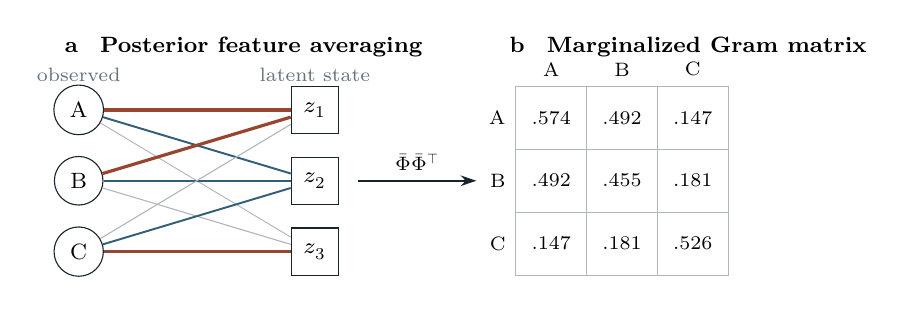
\begin{tikzpicture}[node distance=7mm]
  \node[font=\footnotesize\bfseries,anchor=west] at (-.3,2.5)
    {a\quad Posterior feature averaging};
  \foreach \y/\name in {1.7/A,.8/B,-.1/C}
    \node[draw=BookInk,circle,minimum size=6mm,font=\footnotesize] (o\name) at (0,\y) {\name};
  \foreach \y/\name in {1.7/1,.8/2,-.1/3}
    \node[draw=BookInk,rectangle,minimum size=6mm,font=\footnotesize] (z\name) at (3,\y) {$z_\name$};
  \draw[BookRed,line width=1.4pt] (oA)--(z1);
  \draw[BookBlue,line width=.7pt] (oA)--(z2);
  \draw[BookRule,line width=.35pt] (oA)--(z3);
  \draw[BookRed,line width=1.15pt] (oB)--(z1);
  \draw[BookBlue,line width=.9pt] (oB)--(z2);
  \draw[BookRule,line width=.4pt] (oB)--(z3);
  \draw[BookRule,line width=.4pt] (oC)--(z1);
  \draw[BookBlue,line width=.7pt] (oC)--(z2);
  \draw[BookRed,line width=1.35pt] (oC)--(z3);
  \node[book/note] at (0,2.15) {observed};
  \node[book/note] at (3,2.15) {latent state};
  \draw[book/arrow] (3.55,.8)--(5.05,.8)
    node[midway,above,font=\scriptsize] {$\bar\Phi\bar\Phi^\top$};
  \node[font=\footnotesize\bfseries,anchor=west] at (5.35,2.5)
    {b\quad Marginalized Gram matrix};
  \matrix (gram) [matrix of nodes,nodes={minimum width=9mm,minimum height=8mm,
      draw=BookRule,line width=.35pt,font=\scriptsize},
      row sep=-\pgflinewidth,column sep=-\pgflinewidth] at (6.9,.8) {
    .574 & .492 & .147\\
    .492 & .455 & .181\\
    .147 & .181 & .526\\
  };
  \foreach \j/\lab in {1/A,2/B,3/C}
    \node[font=\scriptsize,anchor=south] at (gram-1-\j.north) {\lab};
  \foreach \i/\lab in {1/A,2/B,3/C}
    \node[font=\scriptsize,anchor=east] at (gram-\i-1.west) {\lab};
\end{tikzpicture}
\end{document}
